\section{Introduction}
\label{sec:intro}

Diffusion probabilistic models \citep{sohldickstein2015nonequilibrium} have recently emerged as the de facto standard for generative modeling in continuous domains.
Their flexibility in representing complex, high-dimensional distributions has led to the adoption of diffusion models in applications including image and video synthesis \citep{ramesh2021dalle,saharia2022imagen,ho2022imagenvideo}, drug and material design \citep{xu2021geodiff,xie2021crystal,schneuing2022structure}, and continuous control \citep{janner2022diffuser,wang2022dql,hansenestruch2023idql}.
The key idea behind diffusion models is to iteratively transform a simple prior distribution into a target distribution by applying a sequential denoising process.
This procedure is conventionally motivated as a maximum likelihood estimation problem, with the objective derived as a variational lower bound on the log-likelihood of the training data.

However, most use cases of diffusion models are not directly concerned with likelihoods, but instead with downstream objective such as human-perceived image quality or drug effectiveness.
In this paper, we consider the problem of training diffusion models to satisfy such objectives directly, as opposed to matching a data distribution.
This problem is challenging because exact likelihood computation with diffusion models is intractable, making it difficult to apply many conventional reinforcement learning (RL) algorithms.
We instead propose to frame denoising as a multi-step decision-making task, using the exact likelihoods at each denoising step in place of the approximate likelihoods induced by a full denoising process.
We present a policy gradient algorithm, which we refer to as \methodfull{} (\methodours{}), that can optimize a diffusion model for downstream tasks using only a black-box reward function.

We apply our algorithm to the finetuning of large text-to-image diffusion models.
Our initial evaluation focuses on tasks that are difficult to specify via prompting, such as image compressibility, and those derived from human feedback, such as aesthetic quality.
However, because many reward functions of interest are difficult to specify programmatically, finetuning procedures often rely on large-scale human labeling efforts to obtain a reward signal \citep{ouyang2022instructgpt}.
In the case of text-to-image diffusion, we propose a method for replacing such labeling with feedback from a vision-language model (VLM).
Similar to RLAIF finetuning for language models \citep{bai2022constitutional}, the resulting procedure allows for diffusion models to be adapted to reward functions that would otherwise require additional human annotations.
We use this procedure to improve prompt-image alignment for unusual subject-setting compositions.

Our contributions are as follows.
We first present the derivation and conceptual motivation of \methodours{}.
We then document the design of various reward functions for text-to-image generation, ranging from simple computations to workflows involving large VLMs, and demonstrate the effectiveness of \methodours{} compared to alternative reward-weighted likelihood methods in these settings.
Finally, we demonstrate the generalization ability of our finetuning procedure to unseen prompts.

\begin{figure}
    \centering
    \begin{minipage}{\linewidth}
            {
                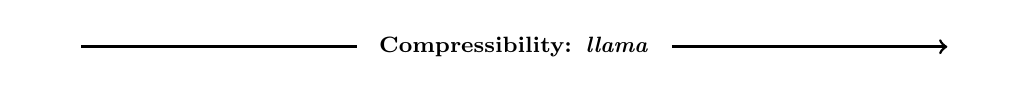
\begin{tikzpicture}
                    \draw[-, line width=1pt] (-5.5,0) -- (-2.0,0);
                    \node[text width=\linewidth, align=center] at (0,0) {
                        \footnotesize
                        \text{\textbf{Compressibility: \emph{llama}}}
                    };
                    \draw[->, line width=1pt] (2.0,0) -- (5.5,0);
                \end{tikzpicture} \\
            }
        \lfbox[
            border-width=2pt,
            padding-top=0pt,
            padding-bottom=0pt,
            padding-left=-2.6pt,
            padding-right=-2.5pt,
        ]{
            \includegraphics*[width=0.1684\linewidth]{teaser/jpeg-ppo-llama/0.jpg}
            \hspace{-0.7em}
            \includegraphics*[width=0.1684\linewidth]{teaser/jpeg-ppo-llama/9.jpg}
            \hspace{-0.7em}
            \includegraphics*[width=0.1684\linewidth]{teaser/jpeg-ppo-llama/39.jpg}
            \hspace{-0.7em}
            \includegraphics*[width=0.1684\linewidth]{teaser/jpeg-ppo-llama/59.jpg}
            \hspace{-0.7em}
            \includegraphics*[width=0.1684\linewidth]{teaser/jpeg-ppo-llama/79.jpg}
            \hspace{-0.7em}
            \includegraphics*[width=0.1684\linewidth]{teaser/jpeg-ppo-llama/99.jpg}
        }
    \end{minipage}
    \vspace{0.1em} \\
    \begin{minipage}{\linewidth}
        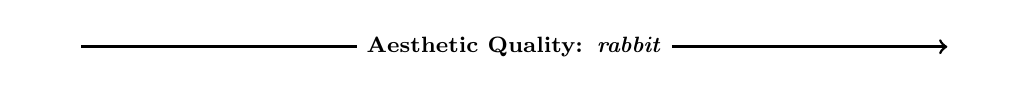
\begin{tikzpicture}
            \draw[-, line width=1pt] (-5.5,0) -- (-2,0);
            \node[text width=\linewidth, align=center] at (0,0) {
                \footnotesize
                \text{\textbf{Aesthetic Quality: \emph{rabbit}}}
            };
            \draw[->, line width=1pt] (2,0) -- (5.5,0);
        \end{tikzpicture} \\
        \lfbox[
            border-width=2pt,
            padding-top=0pt,
            padding-bottom=0pt,
            padding-left=-2.6pt,
            padding-right=-2.5pt,
        ]{
            \includegraphics*[width=0.1684\linewidth]{teaser/rabbit-aesthetic/0.jpg}
            \hspace{-0.7em}
            \includegraphics*[width=0.1684\linewidth]{teaser/rabbit-aesthetic/1.jpg}
            \hspace{-0.7em}
            \includegraphics*[width=0.1684\linewidth]{teaser/rabbit-aesthetic/2.jpg}
            \hspace{-0.7em}
            \includegraphics*[width=0.1684\linewidth]{teaser/rabbit-aesthetic/3.jpg}
            \hspace{-0.7em}
            \includegraphics*[width=0.1684\linewidth]{teaser/rabbit-aesthetic/4.jpg}
            \hspace{-0.7em}
            \includegraphics*[width=0.1684\linewidth]{teaser/rabbit-aesthetic/5.jpg}
        }
    \end{minipage}
    \vspace{0.1em} \\
    \begin{minipage}{\linewidth}
        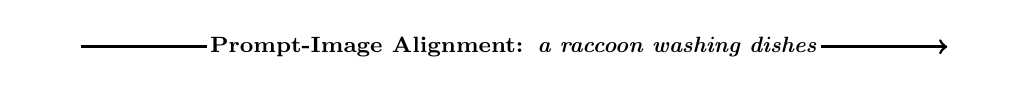
\begin{tikzpicture}
            \draw[-, line width=1pt] (-5.5,0) -- (-3.9,0);
            \node[text width=\linewidth, align=center] at (0,0) {
                \footnotesize
                \text{\textbf{Prompt-Image Alignment: \emph{a raccoon washing dishes}}}
            };
            \draw[->, line width=1pt] (3.9,0) -- (5.5,0);
        \end{tikzpicture} \\
        \lfbox[
            border-width=2pt,
            padding-top=0pt,
            padding-bottom=0pt,
            padding-left=-2.6pt,
            padding-right=-2.5pt,
        ]{
            \includegraphics*[width=0.1684\linewidth]{teaser/raccoon_dishes/0.jpg}
            \hspace{-0.7em}
            
\includegraphics[width=0.1684\linewidth]{teaser/raccoon_dishes/1.jpg}
            \hspace{-0.7em}
            \includegraphics*[width=0.1684\linewidth]{teaser/raccoon_dishes/2.jpg}
            \hspace{-0.7em}
            \includegraphics*[width=0.1684\linewidth]{teaser/raccoon_dishes/3.jpg}
            \hspace{-0.7em}
            \includegraphics*[width=0.1684\linewidth]{teaser/raccoon_dishes/4.jpg}
            \hspace{-0.7em}
            \includegraphics*[width=0.1684\linewidth]{teaser/raccoon_dishes/5.jpg}
        }
    \end{minipage}
    \caption{
        \textbf{(Reinforcement learning for diffusion models)}
            We propose a reinforcement learning algorithm, \methodours{}, for optimizing diffusion models on downstream objectives such as compressibility, aesthetic quality, and prompt-image alignment as determined by vision-language models. Each row shows a progression of samples for the same prompt and random seed over the course of training.
        }
    \vspace{-10pt}
\end{figure}
